\documentclass[border=2pt]{standalone}
\usepackage{tikz}
\usepackage{lmodern}
\renewcommand{\familydefault}{\sfdefault}
\usetikzlibrary{calc}
% Data: Stage-A binary gate (n=3,669)
\begin{document}
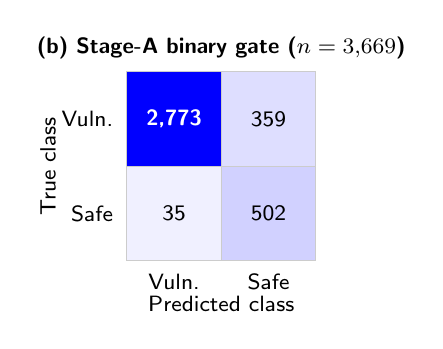
\begin{tikzpicture}[font=\footnotesize\sffamily]
  \def\bs{1.2}
  \foreach \r/\row in {0/{2773,359},1/{35,502}}{
    \foreach \v [count=\c from 0] in \row {
      \pgfmathsetmacro{\shade}{min(100,\v/2773*100)}
      \pgfmathsetmacro{\shade}{max(\shade,6)}
      \fill[blue!\shade!white] (\c*\bs,-\r*\bs) rectangle ++(\bs,-\bs);
      \draw[gray!40] (\c*\bs,-\r*\bs) rectangle ++(\bs,-\bs);
    }
  }
  \node[white,font=\footnotesize\bfseries\sffamily] at (0.5*\bs,-0.5*\bs) {2{,}773};
  \node[font=\footnotesize\sffamily] at (1.5*\bs,-0.5*\bs) {359};
  \node[font=\footnotesize\sffamily] at (0.5*\bs,-1.5*\bs) {35};
  \node[font=\footnotesize\sffamily] at (1.5*\bs,-1.5*\bs) {502};
  \node[anchor=east] at (-0.05,-0.5*\bs) {Vuln.};
  \node[anchor=east] at (-0.05,-1.5*\bs) {Safe};
  \node[anchor=north] at (0.5*\bs,-2*\bs-0.05) {Vuln.};
  \node[anchor=north] at (1.5*\bs,-2*\bs-0.05) {Safe};
  \node at (\bs,-2*\bs-0.55) {Predicted class};
  \node[rotate=90] at (-1.0,-\bs) {True class};
  \node[font=\footnotesize\bfseries\sffamily,align=center] at (\bs,0.3) {(b) Stage-A binary gate ($n=3{,}669$)};
\end{tikzpicture}
\end{document}
